\documentclass[12pt]{article}

%==============================
%        PACOTES BÁSICOS
%==============================
\usepackage[utf8]{inputenc}
\usepackage[T1]{fontenc}
\usepackage[brazil]{babel}
\usepackage[useregional]{datetime2}
\usepackage{graphicx}
\usepackage{amsmath, amssymb}
\usepackage{setspace}
\usepackage{enumitem}
\usepackage[colorlinks=true, linkcolor=black, urlcolor=blue, citecolor=black]{hyperref}
\usepackage{caption}
\usepackage{parskip}
\usepackage{float}
\usepackage{ragged2e}
\usepackage{helvet}
\renewcommand{\familydefault}{\sfdefault}
\usepackage{titlesec}
\usepackage[a4paper, top=2cm, bottom=2.5cm, left=3cm, right=2cm]{geometry}
\usepackage{tcolorbox}

\usepackage{circuitikz}

\usepackage{tabularx}
\usepackage{array, xcolor, booktabs}
\usepackage[table]{xcolor}
\usepackage{multirow}

%==============================
%      INDENTAÇÃO ABNT
%==============================
\usepackage{indentfirst}
\setlength{\parindent}{1.25cm}

%==============================
%      ESTILO DAS SECTIONS
%==============================
%gostaria que tivesse com o /newpage no final automático

%==============================
%        DOCUMENTO
%==============================
\begin{document}

%==============================
%            CAPA
%==============================
\begin{titlepage}
\thispagestyle{empty}
\centering

{\large Escola Politécnica da Universidade de São Paulo\par}
\vspace{1.2em}

{\large \textbf{PCS3115} -- Sistemas Digitais II (2026)\par}
\vspace{5em}

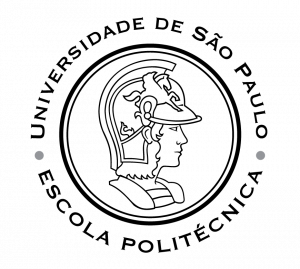
\includegraphics[width=0.4\textwidth]{logo.png}
\vspace{4em}

{\Large\bfseries Relatório da Atividade Formativa I\par}
\vspace{4em}

{\Large Turma: 1/3\par}
Professor(es): Antonio Vieira da Silva Neto

\vfill

\begin{center}
Victor Augusto D M N da Silva (NUSP: 16903351)\\
Enzo Ashikawa Cabas (NUSP: 15520151)\\
Pedro Meira de Lima (NUSP: 16835748)\\
Luiz Felipe Dias Alves (NUSP: 16819249)\\
ahmed lima trovão (NUSP: 13681335)\\
César Silvestre Campos (NUSP: 16860413)

\end{center}

\vspace{1em}
{\large São Paulo, \the\year\par}

\end{titlepage}

%==============================
%          SEÇÕES
%==============================
\section{EXERCÍCIO 1: ANÁLISE DE CIRCUITOS COMBINATÓRIOS}

\begin{tcolorbox}[title=Enunciado da Questão,colback=gray!5,colframe=black]

Gabriel sempre foi um sonhador. Desde pequeno, queria ser um herói porque
assistia a filmes em que, nos momentos de dificuldade, o herói sempre salvava a todos.
Após uma longa e árdua graduação, Gabriel viu-se em uma grande inquietação: o que fazer
agora da vida?

Por um lado, ele estava muito bem empregado como engenheiro em uma grande
multinacional; por outro, ele sentia que algo faltava em sua vida. Foi, então, que ele se
lembrou de um presente que havia recebido no dia de sua formatura. Seus professores da
disciplina de Sistemas Digitais, Felipe e Antônio, entregaram-lhe uma caixa embrulhada
e disseram que, quando sentisse que a hora certa chegasse, ele deveria abrir a caixa.

Após muito procurar, ele finalmente encontrou o embrulho, embaixo de vários livros
de Cálculo, Física e Álgebra Linear. Após remover o embrulho, ele percebeu que, colado
na caixa, havia um bilhete com a seguinte mensagem: “A jornada da perfeição inicia-se com um único passo.”.

A caixa estava trancada por um cadeado com quatro senhas, sendo cada senha um
número decimal que varia entre 00 e 15. Na parte superior da caixa, havia o circuito digital
da Figura 1. Lembrando dos conhecimentos adquiridos na disciplina de Sistemas Digitais,
Gabriel deduziu que deveria existir uma relação entre o conjunto de entradas ABCD e as
senhas do cadeado. Ele realizou, então, o processo de análise do circuito combinatório
para descobrir a senha

\begin{figure}[H]
\centering
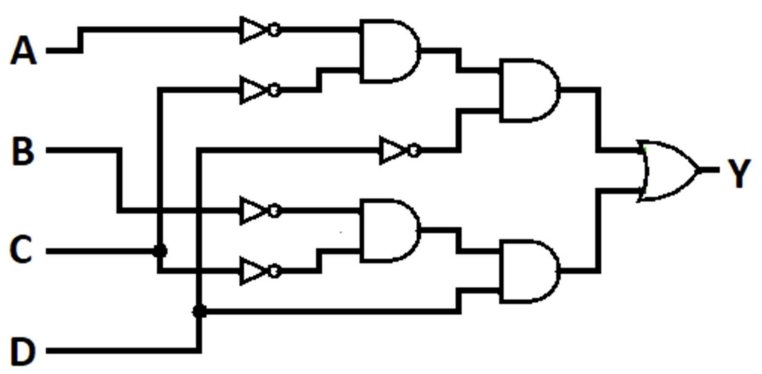
\includegraphics[width=0.5\textwidth, angle=0]{Captura de tela 2026-03-16 154834.png}
\caption{Circuito do exercício.}
\label{fig:circuito_novo}
\end{figure}

\end{tcolorbox}

\subsection{Pergunta (a)}

\subsubsection*{Enunciado}
Monte e preencha a tabela verdade do “circuito desconhecido”.

\subsubsection*{Resposta}

Primeiro, para tornar a tabela verdade de maneira mais eficiente, encontra-se a expressão lógica que representa esse circuito combinatório:

\begin{equation}
Y = [(\overline{A} \cdot \overline{C}) \cdot \overline{D}] + [(\overline{B} \cdot \overline{C}) \cdot D]
\label{equação lógica 1}
\end{equation}

Assim, monta-se a tabela verdade com as quatro entradas e as partes relevantes:

\begin{table}[H]
\caption{Tabela-verdade}
\centering
\renewcommand{\arraystretch}{1.3}
\begin{tabular}{|c|c|c|c|c|c|c|}
    \hline
    A & B & C & D & $(\overline{A} \cdot \overline{C}) \cdot \overline{D}$ & $(\overline{B} \cdot \overline{C}) \cdot D$  & Y\\
    \hline
    0 & 0 & 0 & 0 & 1 & 0 & 1 \\
0 & 0 & 0 & 1 & 0 & 1 & 1 \\
0 & 0 & 1 & 0 & 0 & 0 & 0 \\
0 & 0 & 1 & 1 & 0 & 0 & 0 \\
0 & 1 & 0 & 0 & 1 & 0 & 1 \\
0 & 1 & 0 & 1 & 0 & 0 & 0 \\
0 & 1 & 1 & 0 & 0 & 0 & 0 \\
0 & 1 & 1 & 1 & 0 & 0 & 0 \\
1 & 0 & 0 & 0 & 0 & 0 & 0 \\
1 & 0 & 0 & 1 & 0 & 1 & 1 \\
1 & 0 & 1 & 0 & 0 & 0 & 0 \\
1 & 0 & 1 & 1 & 0 & 0 & 0 \\
1 & 1 & 0 & 0 & 0 & 0 & 0 \\
1 & 1 & 0 & 1 & 0 & 0 & 0 \\
1 & 1 & 1 & 0 & 0 & 0 & 0 \\
1 & 1 & 1 & 1 & 0 & 0 & 0 \\
\hline
\end{tabular}
\end{table}

\subsection{Pergunta (b)}

\subsubsection*{Enunciado}
Apresente a equação que relaciona a saída Y com as entradas A, B, C e D
por meio da forma canônica da soma de mintermos.

\subsubsection*{Resposta}
Os mintermos correspondem às combinações de entrada para as quais a saída assume valor 1. Cada mintermo é formado escrevendo-se a variável direta (ela mesma) quando seu valor é 1 e seu complemento quando é 0.

A partir da tabela-verdade, observa-se que a saída vale 1 para as combinações:

\[
\begin{array}{cc}
0000 \rightarrow m_0 \ \ \ & \ \ \ 0001 \rightarrow m_1 \\
0100 \rightarrow m_4 \ \ \ & \ \ \ 1001 \rightarrow m_9
\end{array}
\]

Assim, cada uma das linhas que dão 1 gera um produto dos mintermos:

\[
\begin{array}{cc}
m_0 = \overline{A}\,\overline{B}\,\overline{C}\,\overline{D}
\ \ \ & \ \ \ 
m_1 = \overline{A}\,\overline{B}\,\overline{C}\,D
\\[0.4em]
m_4 = \overline{A}\,B\,\overline{C}\,\overline{D}
 \ \ \ & \ \ \ 
m_9 = A\,\overline{B}\,\overline{C}\,D
\end{array}
\]

A soma lógica desses mintermos produz a forma "canônica" da função:

\begin{equation}
Y = \overline{A} \ \overline{B} \ \overline{C} \ \overline{D} + \overline{A} \ \overline{B} \ \overline{C} \ D + \overline{A} \ B \ \overline{C} \ \overline{D} + A \ \overline{B} \ \overline{C} \ D
\label{equação lógica 2}
\end{equation}

\subsection{Pergunta (c)}

\subsubsection*{Enunciado}
Considerando que o conjunto de entradas ABCD representa um número
na base decimal, indique qual a função do circuito. Quais são as quatro senhas
necessárias para destravar o cadeado da caixa?

\subsubsection*{Resposta}

Considera-se as entradas $A$, $B$, $C$ e $D$ como um número binário de quatro algarismos, em que $A$ é o mais significativo e $D$ o menos significativo. Assim, cada combinação representa um número binário, e este um decimal dentro do intervalo dos naturais:

\[
\{0,1,2,\dots,15\}
\]

A partir da tabela-verdade de (a), observa-se que a saída assume valor 1 apenas para os valores:

\[
0000,\;0001,\;0100,\;1001
\]

que correspondem, em decimal, a:

\[
0,\;1,\;4,\;9
\]

Percebe-se, depois de certo ponderamento, que esses valores são exatamente os quadrados perfeitos existentes no intervalo de 0 a 15.
Portanto, o circuito funciona como um \textbf{detector de quadrados perfeitos em números binários de quatro bits} e pode ser definida por:

\[
f:\{0,1,\dots,15\}\to\{0,1\}
\]

tal que

\[
f(x)=
\begin{cases}
1, & \text{se } x \in \{0,1,4,9\} \ \ \lor  \ \ x \in \{ quadrados  \ \ perfeitos \}\\
0, & \text{caso contrário}
\end{cases}
\]


Assim, as quatro senhas necessárias para destravar o cadeado são:

\[
\boxed{0,\;1,\;4,\;9}
\]

\section{EXERCÍCIO 2: ÁLGEBRA BOOLEANA}

\begin{tcolorbox}[title=Enunciado da Questão,colback=gray!5,colframe=black]
Após destravar a caixa, Gabriel encontrou dentro dela um tabuleiro com diversas
peças, que representam as portas lógicas AND, OR, NOT, NAND e NOR. Além do tabuleiro
e das peças, havia também um novo bilhete com a seguinte mensagem: “Às vezes os
problemas que queremos resolver não possuem somente uma solução, mas duas, ou até
três!”.

Inicialmente, Gabriel tentou montar um circuito idêntico ao que estava no topo da
caixa, mas nada aconteceu. Foi então que ele percebeu que havia espaço o suficiente para
montar dois circuitos no tabuleiro com as seguintes inscrições: “dual” e “NAND only”. Siga
o raciocínio de Gabriel e elabore os seguintes circuitos combinatórios:
\end{tcolorbox}

\subsection{Pergunta (a)}

\subsubsection*{Enunciado}
Apresente a versão dual do circuito da Figura 1. O que acontece com a
interpretação das entradas e saídas da versão dual em comparação com o circuito
original? 

\subsubsection*{Resposta}

A expressão lógica original obtida no Exercício 1 foi:

\begin{equation}
Y = [(\overline{A}\cdot\overline{C})\cdot\overline{D}] + [(\overline{B}\cdot\overline{C})\cdot D]
\label{eq:original}
\end{equation}

Para obter a forma dual, aplica-se o princípio da dualidade da álgebra booleana, segundo o qual:

\begin{itemize}
    \item cada operação AND ($\cdot$) é substituída por OR ($+$), e o contrário;
    \item cada operação 0 é substituída por 1 na tabela verdade, e o contrário;
    \item a tabela verdade do resultado é flipada verticalmente;
\end{itemize}

Assim, podemos deduzir a regra conhecida de que s complementos permanecem inalterados e a expressão dual torna-se:

\begin{equation}
Y_d = [(\overline{A}+\overline{C})+\overline{D}] \cdot [(\overline{B}+\overline{C})+D]
\label{eq:dual}
\end{equation}

A Figura \ref{fig:circuito_dual} apresenta o circuito correspondente à expressão dual:

\begin{figure}[H]
\centering
\begin{circuitikz}[american, transform shape]

% Entradas
\draw
(0,6) node[left] {$A$} -- (1,6)
(0,4) node[left] {$B$} -- (1,4)
(0,2) node[left] {$C$} -- (1,2)
(0,0) node[left] {$D$} -- (1,0);

% Inversores
\draw
(1.2,6) node[not port, scale=0.5] (notA) {}
(1.2,4) node[not port, scale=0.5] (notB) {}
(1.2,2) node[not port, scale=0.5] (notC) {}
(3.5,0) node[not port, scale=0.5] (notD) {};

% Fios após inversores
\draw
(notA.out) -- (2,6)
(notB.out) -- (2.2,4)
(notC.out) -- (2.2,2)
(1,0) -- (3.15,0)
(notD.out) -- (4.2,0);

% OR superior esquerda: A' + C'
\draw
(3.4,5) node[or port, scale=0.7] (or1) {};

\draw
(2,6) |- (or1.in 1)
(2,2) |- (or1.in 2);

% OR superior direita: (A'+C') + D'
\draw
(5.5,4.8) node[or port, scale=0.7] (or2) {};

\draw
(or1.out) -- (or2.in 1)
(4.2,0) |- (or2.in 2);

% OR inferior esquerda: B' + C'
\draw
(3.4,3) node[or port, scale=0.7] (or3) {};

\draw
(2.2,4) |- (or3.in 1)
(2.2,2) |- (or3.in 2);

% OR inferior direita: (B'+C') + D
\draw
(5.5,2.8) node[or port, scale=0.7] (or4) {};

\draw
(or3.out) -- (or4.in 1)
(3,0) |- (or4.in 2);

%node indicators 
\draw
(3,0) node[fill, circle, inner sep=1.2pt] (nodeD) {}
(2,2) node[fill, circle, inner sep=1.2pt] (nodeC) {};

% AND final
\draw
(7.5,3.75) node[and port, scale=0.7] (and1) {};

\draw
(or2.out) -- (and1.in 1)
(or4.out) -- (and1.in 2);

% Saída
\draw
(and1.out) -- (8.5,3.75) node[right] {$Y_d$};

\end{circuitikz}
\caption{Circuito dual obtido a partir da expressão lógica original.}
\label{fig:circuito_dual}
\end{figure}

A tabela-verdade correspondente ao circuito dual é apresentada a seguir:

\begin{table}[H]
\centering

\renewcommand{\arraystretch}{1.2}
\begin{tabular}{|c|c|c|c|c|}
\hline
A & B & C & D & $Y_d$ \\
\hline
0 & 0 & 0 & 0 & 1 \\
0 & 0 & 0 & 1 & 1 \\
0 & 0 & 1 & 0 & 0 \\
0 & 0 & 1 & 1 & 1 \\
0 & 1 & 0 & 0 & 1 \\
0 & 1 & 0 & 1 & 0 \\
0 & 1 & 1 & 0 & 0 \\
0 & 1 & 1 & 1 & 0 \\
1 & 0 & 0 & 0 & 1 \\
1 & 0 & 0 & 1 & 1 \\
1 & 0 & 1 & 0 & 0 \\
1 & 0 & 1 & 1 & 0 \\
1 & 1 & 0 & 0 & 0 \\
1 & 1 & 0 & 1 & 0 \\
1 & 1 & 1 & 0 & 0 \\
1 & 1 & 1 & 1 & 0 \\
\hline
\end{tabular}
\caption{Tabela-verdade do circuito dual}
\end{table}

Comparando-se com o circuito original, observa-se que a versão dual altera o comportamento lógico da saída:

\begin{itemize}
    \item Primeiro, o circuito sai de active high para active low.
    \item no circuito original, a saída é ativada apenas para alguns mintermos específicos. Enquanto no circuito dual, novas combinações de entrada passam a satisfazer a função lógic.
\end{itemize}

Portanto, a versão dual não preserva a função do circuito original, mas mantém a estrutura algébrica correspondente à dualidade da lógica booleana.

\subsection{Pergunta (b)}

\subsubsection*{Enunciado}
Apresente uma versão equivalente do circuito da Figura 1 utilizando somente portas NAND. 

\subsubsection*{Resposta}

Partindo da expressão original:

\begin{equation}
Y = [(\overline{A}\cdot\overline{C}) \cdot \overline{D}] + [(\overline{B}\cdot\overline{C}) \cdot D]
\end{equation}

Aplicando o teorema de De Morgan:

\begin{equation}
Y=
\overline{
\overline{[(\overline{A}\cdot\overline{C})\cdot\overline{D}]}
\cdot
\overline{[(\overline{B}\cdot\overline{C})\cdot D]}
}
\end{equation}

A Figura \ref{fig:circuito_nand} apresenta o circuito equivalente do circuito da figura \ref{eq:original}, feita com a fórmula que chegamos usando De Morgan e com o que sabemos de como calcular portas lógicas à partir das portas nand: NOT = (Nand com o fio nos dois terminais), AND = (NAND -> NOT feito com NAND) e OR = (Nots feitos com NAND => NAND), o que culminou no seguinte circuito:

\begin{figure}[H]
\centering
\begin{circuitikz}[american, transform shape]

% Entradas
\draw
(0,6) node[left] {$A$} -- (1,6)
(0,4) node[left] {$B$} -- (1,4)
(0,2) node[left] {$C$} -- (1,2)
(0,0) node[left] {$D$} -- (3.3,0);

% Inversores com nand iniciais
\draw
(1.5,6) node[nand port, scale=0.35] (nandA) {}
(1.5,4) node[nand port, scale=0.35] (nandB) {}
(1.5,2) node[nand port, scale=0.35] (nandC) {}
(3.8,0) node[nand port, scale=0.35] (nandD) {};

% Fios que conectam os terminais dos inversores NAND
% A
\draw (1,6) |- (nandA.in 1);
\draw (1,6) |- (nandA.in 2);
% B
\draw (1,4) |- (nandB.in 1);
\draw (1,4) |- (nandB.in 2);
% C
\draw (1,2) |- (nandC.in 1);
\draw (1,2) |- (nandC.in 2);
% D
\draw (3.3,0) |- (nandD.in 1);
\draw (3.3,0) |- (nandD.in 2);

% Fios após inversores com nand
\draw
(nandA.out) -- (2,6)
(nandB.out) -- (2.2,4)
(nandC.out) -- (2.2,2)
(nandD.out) -- (4.2,0);

% OR superior esquerda: A' + C'
\draw
(3.4,5) node[nand port, scale=0.7] (nandAC) {};

%conexão segunda parte dos fios com nand até os nands principais inciciais
\draw
(2,6) |- (or1.in 1)
(2,2) |- (or1.in 2);

% OR superior direita: (A'+C') + D'
\draw
(5.5,4.8) node[nand port, scale=0.7] (nandBC) {};

\draw
(4,5) -- (4.7,5)
(4.2,0) |- (or2.in 2);

% OR inferior esquerda: B' + C'
\draw
(3.4,3) node[nand port, scale=0.7] (nandACD) {};

\draw
(2.2,4) |- (or3.in 1)
(2.2,2) |- (or3.in 2);

% OR inferior direita: (B'+C') + D
\draw
(5.5,2.8) node[nand port, scale=0.7] (nandBCD) {};

\draw
(4,3) -- (4.7,3)
(3,0) |- (or4.in 2);

% inversores nand para corrigir para and
\draw
(4,5) node[nand port, scale=0.35] (nandNot1) {}
(4,3) node[nand port, scale=0.35] (nandNot2) {};

% Fios que conectam os terminais dos inversores NAND
% Not1
\draw (3.5,5) |- (nandNot1.in 1);
\draw (3.5,5) |- (nandNot1.in 2);
% Not2
\draw (3.5,3) |- (nandNot2.in 1);
\draw (3.5,3) |- (nandNot2.in 2);


%node indicators 
\draw
(3,0) node[fill, circle, inner sep=1.2pt] (nodeD) {}
(2,2) node[fill, circle, inner sep=1.2pt] (nodeC) {};

% NAND final
\draw
(7.5,3.75) node[nand port, scale=0.7] (and1) {};


\draw
(or2.out) -- (and1.in 1)
(or4.out) -- (and1.in 2);

% Saída
\draw
(and1.out) -- (8.5,3.75) node[right] {$Y_d$};

\end{circuitikz}
\caption{Implementação utilizando apenas portas NAND.}
\label{fig:circuito_nand}
\end{figure}

Algo que vale ser comentado é o fato dos Not's depois dos nands que conectam ABD e BCD estarem no mesmo fio dos necessários para a criação do Or com o Nand final, então eles foram "anulados".

Temos, logo, mais um exemplo para aomo qualquer outro desses tipos de circuitos combinatórios, podemos implementá-lo exclusivamente com portas NAND, explorando o fato da porta nand ser "universal".

\end{document}
